\documentclass[a4paper, 12pt]{article}
\usepackage{parskip}   % for formatting paragraphs nicer
\usepackage{graphicx}  % for images
\usepackage{color}
\usepackage{amsmath}   % for text in maths
\usepackage{hyperref}  % hyperlinks, also for links on contents page
\usepackage{textcomp}  % for degree sign

\title{Physics Notes}
\date{}
\begin{document}

\maketitle
\tableofcontents
\newpage

\section{Particles}

\subsection{Classification}

There are two main groups of particles: Hadrons and Leptons.

Hadrons feel the strong force and are made up of quarks. The proton is the only stable baryon, while a neutron left on it's own will decay with a half life of about 11 minutes.

Leptons are fundamental particles like quarks, and do not feel the strong force. They mostly interact through the weak interaction (or EM if charged, and gravitational force as they have mass).
Leptons have a lepton number that is always conserved in a interaction. Neutrinos are leptons and have no charge, and very little mass, so they are hard to detect.

Hadrons consist of two separate families of particles: Baryons and Mesons.

Baryons consist of 3 quarks of any type. Mesons are a quark - anti quark pair.

\begin{center}
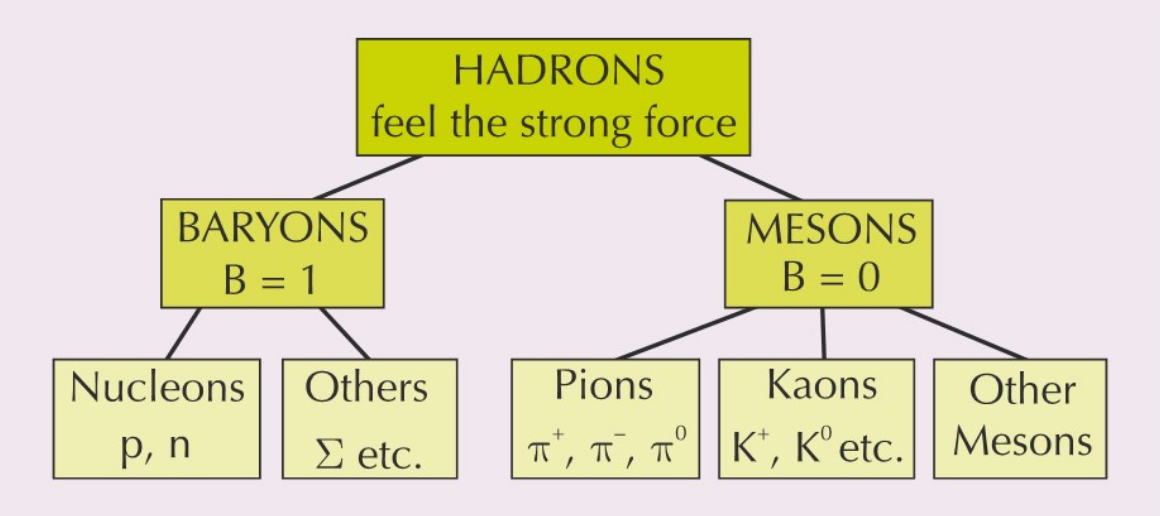
\includegraphics[height=5cm]{images/hadronFamily.png}
\end{center}

\subsection{Quarks}

Quarks are fundamental particles that make up hadrons.

The only three quarks that you need to know for A-Level is the up quark ($u$), down quark ($d$) and the strange quark ($s$).

Here is the table from the formula sheet showing the properties:

\begin{center}
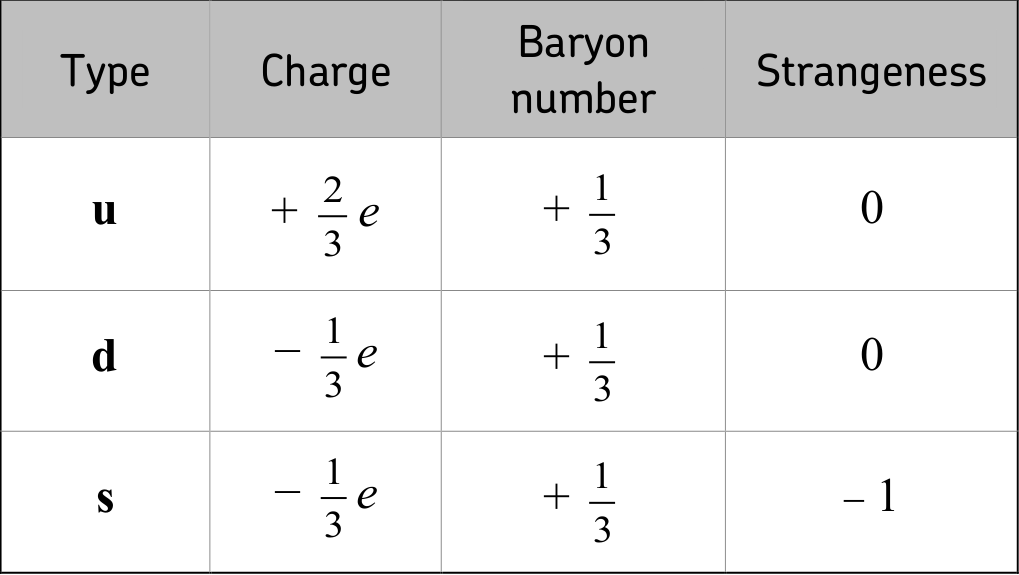
\includegraphics[height=5cm]{images/quarks.png}
\end{center}

\subsubsection{Conservation Laws}

Conserved in all interactions:
\begin{itemize}
	\item{Baryon number}
	\item{Lepton number}
	\item{Momentum}
	\item{Charge}
\end{itemize}

Strangeness is conserved almost all interactions \colorbox{yellow}{unless it is the weak interaction}, as the weak interaction involves changing the type of a quark.

\subsubsection{Specific Charge}

Specific Charge $= \frac{mass}{charge}$

\subsection{Forces}

\subsubsection{Strong Force}

The strong force binds all the nucleons in the nucleus together. It only works between hadrons.

The strong force is {\textbf{repulsive}} at distances $< 0.5$ fm, and {\textbf{attractive}} at distances $> 0.5$ fm to $3$ fm.

The strong force in the nucleus has to be stronger overall (hence the name) than the EM force to keep the nucleus together, as the protons in the nucleus are all repelling each other proton in the nucleus, where as the strong force is much more attractive for the nucleons around it, but has pretty much no effect on other nucleons.

The exchange particle for the strong force is the $\pi$ pion (a meson). (it is actually gluons but we have to say pions).


\subsubsection{Electromagnetic Force}

The electromagnetic force acts between charged particles, where $F \propto \frac{1}{r^2}$, (inverse square law) where $r$ is the distance between the centre's of the particles.

The exchange particle for the EM force is the (virtual) photon ($\gamma$), which has no mass, and travels at the speed of light ($\approx 3 \times 10^8$). It has wave-particle duality.

\subsubsection{Weak Force}

The weak force can act between any two particles. The weak force changes the flavour of a quark. This means that a strange quark can be changed into any other quark, so strangeness may not be conserved in weak interactions. It's pretty weak.

The exchange particle for the weak force is the $W^+$ or $W^-$ boson.

\subsubsection{Gravitational Force}

The gravitational force acts between all particles with mass. Like the EM force, it follows an inverse square law: $F \propto \frac{1}{r^2}$

\subsection{Decays}

Here is a graph showing the different isotopes for varying numbers of neutrons and protons, and what decay is likely to happen to each (unless stable):

\begin{center}
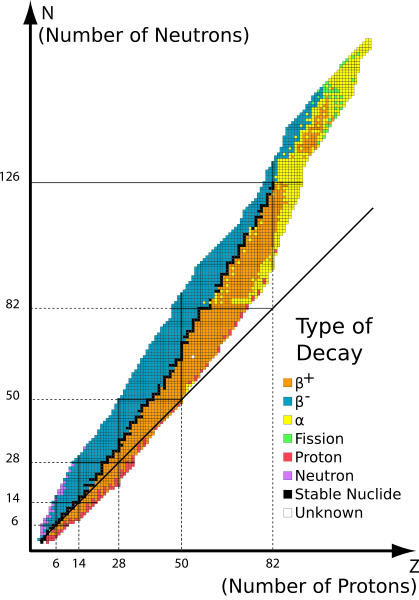
\includegraphics[height=12cm]{images/bandOfStability.png}
\end{center}

At lead ($Pb\, ^{208}_{82}$), 126 neutrons and 82 protons, the stability line ends.

Neon ($Ne\, ^{20}_{10}$) is the last isotope that follows the projection line exactly.

\subsubsection{{$\alpha$} decay}

Alpha decay is the emission of a helium nucleus from an atom's nucleus.

${\alpha^4_2}$

Alpha decay usually happens in very heavy isotopes that need to get rid of both neutrons and protons, due to the EM force in the nucleus overcoming the strong force between nucleons.

An example alpha decay would be:

$Pu^{\,240}_{\,94}\, {\Rightarrow}\, U^{\,236}_{\,92} + \alpha^4_2$

\subsubsection{{$\beta$} decay}

The $\beta$ particle is just a high energy (speed) electron or positron, depending on the charge.

\textbf{$\beta^-$ decay:}

$\beta^-$ decay is when a neutron turns into a proton and electron via the weak interaction. The exchange particle is $W^-$, easy to remember since it is also negative.

Here is the equation for $\beta^-$ decay:

$n^0_1 \, \rightarrow \, p^+_1 + e^- + \overline{V_e}$

The anti neutrino $\overline{V_e}$ is to balance the lepton 

Here is the feynman diagram for $\beta^-$ decay:

\begin{center}
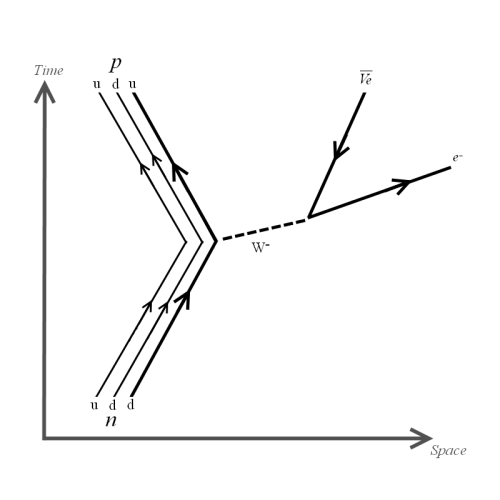
\includegraphics[height=8cm]{images/betaMinus.png}
\end{center}

\textbf{$\beta^+$ decay:}

$\beta^+$ decay is when a proton turns into a neutron and positron. This is key, as the position will annihilate pretty quickly with a nearby electron (as they are antiparticles), producing two high energy photons (probably gamma), so light will be emitted. The exchange particle this time is a $W^+$ boson.

Here is the equation for $\beta^+$ decay:

$p^+_1 \, \rightarrow \, n^0_1 + e^+ + V_e$

Here is the feynman diagram for $\beta^+$ decay:

\begin{center}
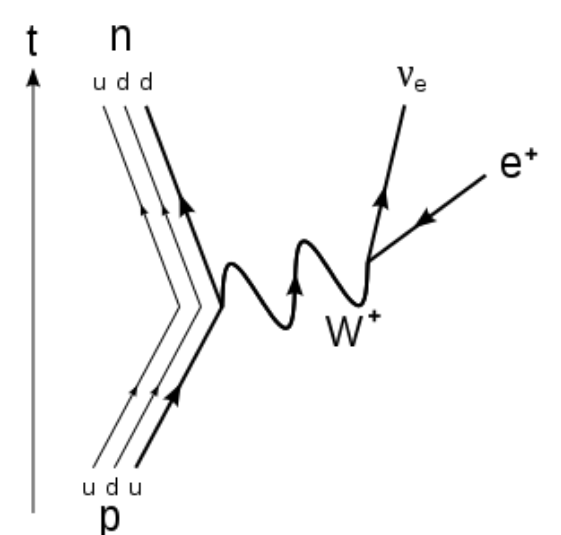
\includegraphics[height=7cm]{images/betaPlus.png}
\end{center}

It is pretty much the reverse of $\beta^-$.

\subsection{Electron Energy Levaels}

Electrons around the nucleus can have different energy levels depending on how far away they are from the nucleus (potential energy). The further away they are from the nucleus, the less energy is required to remove the electron from that energy level and onto a higher one.

\subsection{Pair Production}

If a photon interacts with a nucleus, the energy of the photon can be converted into an electron-positron pair ($energy \rightarrow mass$). This is so that lepton number is conserved.

Here is a diagram:

\begin{center}
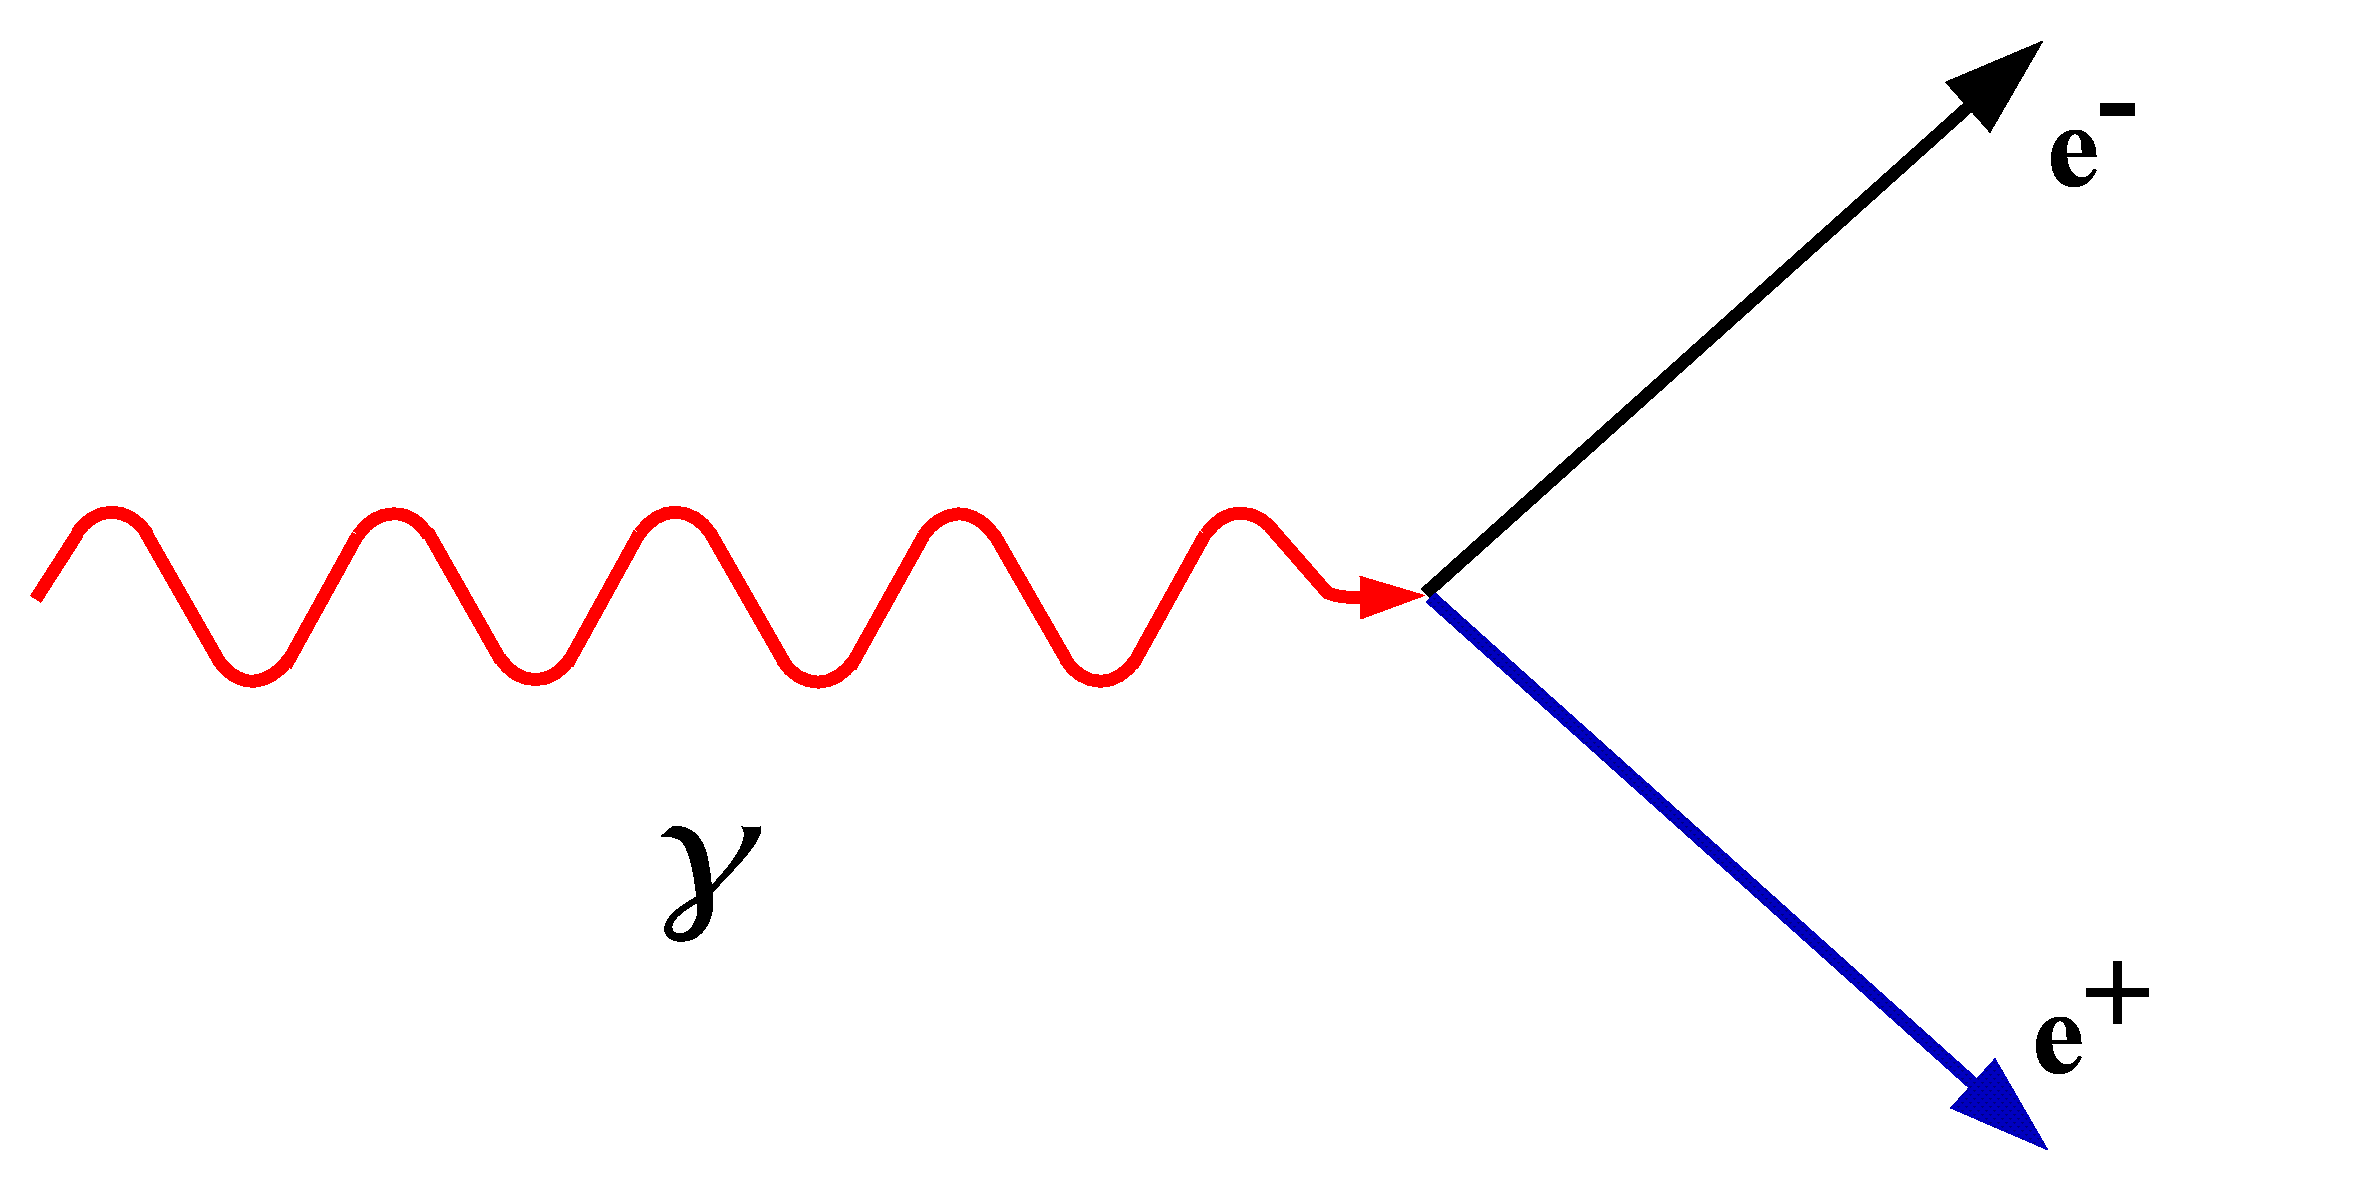
\includegraphics[height=4cm]{images/pairProduction.png}
\end{center}

\subsection{Electron Capture}

Electron capture is when an electron from one of the electron shells is succed into the nucleus, and interacts with a proton in the nucleus to produce a neutron and an electron neutrino. This is pretty much $\beta^+$, but there is no need for a positron since the electron at the start counteracts the charge of the proton at the start, so charge is 0 on both sides.

The equation is:

$p^+_1 + e^-_0 \, \rightarrow \, n^0_1 + Ve^0_0$

\textbf{It is important to remember that a photon will be released when the electron drops down to the ground state.}

\subsection{EM Repulsion}

When two like-charged particles get close, they repel through the EM force. \textbf{Virtual} photons are exchanged during the interaction:

\begin{center}
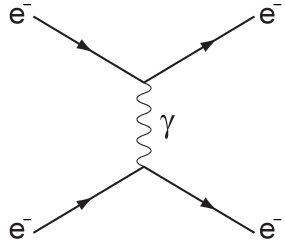
\includegraphics[height=4cm]{images/emRepulsion.png}
\end{center}

\subsection{Antimatter}

Antiparticles have the same attributes as their regular counterparts, but usually the opposite of everything (including charge).

When two antiparticles collide/interact, they annihilate each other, converting the mass of both of the particles into energy in the form of two photons. \colorbox{yellow}{Two photons are produced to conserve momentum.}

Since antiparticles have opposite charges to their normal counterparts, so annihilation is likely to happen if an antiparticle is nearby. Hence why there is so little antimatter compared to matter, but we do not know why there is overall more regular matter than antimatter.
\newpage

\subsection{The Photoelectric Effect}

The photoelectric effect is the process by which a metal with photons incident on it emits electrons (photoelectrons).

The photon interacts with an electron in the metal, and if the photon has enough energy to liberate the electron, then the electron will be liberated. This minimum energy is the work function ($\phi$).

The work function is the minimum energy required to liberate an electron from the \textit{surface} of the material. Electrons from deeper down in the material require more energy to liberate.

The threshold frequency is the frequency of the photon needed to meet that minimum energy requirement (the work function). The equation for the threshold frequency is:
$$
f = \frac{\phi}{h}
$$

Where $\phi$ is the work function of the material, and $h$ is the planck constant.

The equation you get in the equation sheet is:
$$
hf = \phi + E_{k \, (\text{max})}
$$

The photoelectric effect can be demonstrated using a UV lamp and a charged zinc plate and some gold leaf foil:

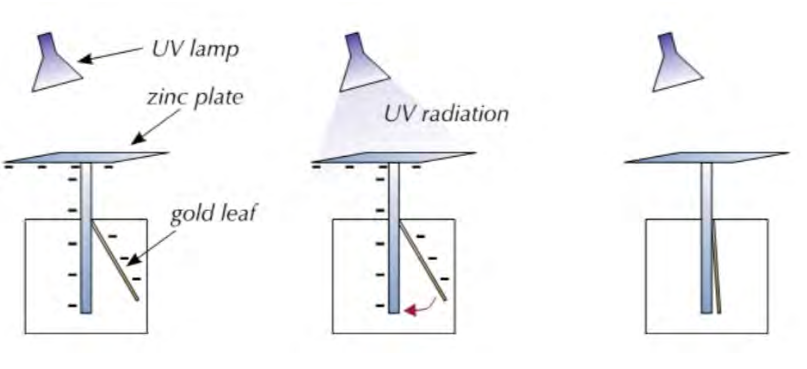
\includegraphics[width=\textwidth]{images/photoelecExp.png}

\newpage
\subsection{Electron Energy Levels}

Around an atom's nucleus there are discrete energy levels.

\textbf{Excitation} is where an electron bound to an atom moves up one or more energy levels. \textbf{De-excitation} is the opposite. Excitation requires energy to move the electron to a higher state, while de-excitation releases energy in the form of a photon.

\textbf{Ionisation} is where the electron is completely removed from the atom.

\subsubsection{Absorption and Emission lines}

The photons absorbed during excitation, or the photons released during de-excitation can be used to figure out what element the substance is made from, as every atom has different energies required to excite/de-excite electrons.

You can make an emission/absorption spectra to find the emission/absorption lines:

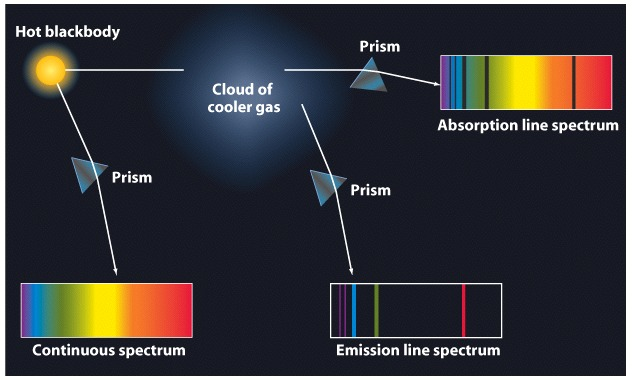
\includegraphics[width=\textwidth]{images/spectraElecEmmision.jpg}

A black body is a body that perfectly absorbs and emits light (if you looked at the spectrum emitted by the black body, you would see no gaps).

\subsubsection{Fluorescent Tubes}

Fluorescent tubes work by firing a beam of free electrons from one end to the other.
The tube is filled with mercury gas, so these free electrons collide with electrons in the atoms in the mercury gas, exciting the electrons. The electrons then de-excite releasing UV photons. There is a phosphorus coating on the inside of the tube, and the UV ray excites electrons in the phosphorus, and quickly de-excites to a lower energy level again, which then releases light in the visible spectrum.

Here is an image of the tube:

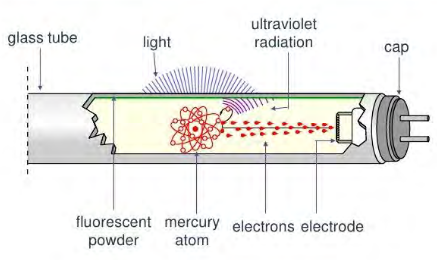
\includegraphics[width=\textwidth]{images/mercuryTube.png}

\subsection{Wave Particle Duality}

Wave particle duality is when a particle has wave-like properties, as well as particle-like qualities. For example, a photon was always thought to be a wave, however the photoelectric effect disproves this, as it requires light to be discrete packets of energy, rather than just a wave.

Another example of wave particle duality would be that electrons can be diffracted if going through a gap of similar size to the De-Broglie wavelength. However, electrons are clearly particles as they are deflected by electric fields, which shows it is also a particle.

Here is the equation for the De-Broglie wavelength:

$$
\lambda = \frac{h}{p} = \frac{h}{mv}
$$

\newpage
\section{Waves}

\subsection{Important Definitions}

\begin{itemize}
	\item{\textbf{Wavelength} $\lambda$ - The length of the wave\dots}
	\item{\textbf{Period} $T$ - The time to complete one wavelength.}
	\item{\textbf{Frequency} $f$ - How many wavelengths received per second, or {$f = \frac{1}{T}$}, where $T$ is the period.}
	\item{\textbf{Displacement} $x$ - The distance from the rest/origin point.}
	\item{\textbf{Amplitude} $A$ - The maximum displacement.}
	\item{\textbf{Phase} - A measurement of the position of a certaain point along the wave cycle.}a
	\item{\textbf{Intensity} - The intensity of light is the number of photons incident per second.}
\end{itemize}

\subsection{Transverse and Longitudinal}

Transverse waves are waves where the oscillation is perpendicular to the direction of propagation. Longitudinal waves are waves where the oscillation is parallel to the direction of propagation.

Transverse vs longitudinal:

\begin{center}
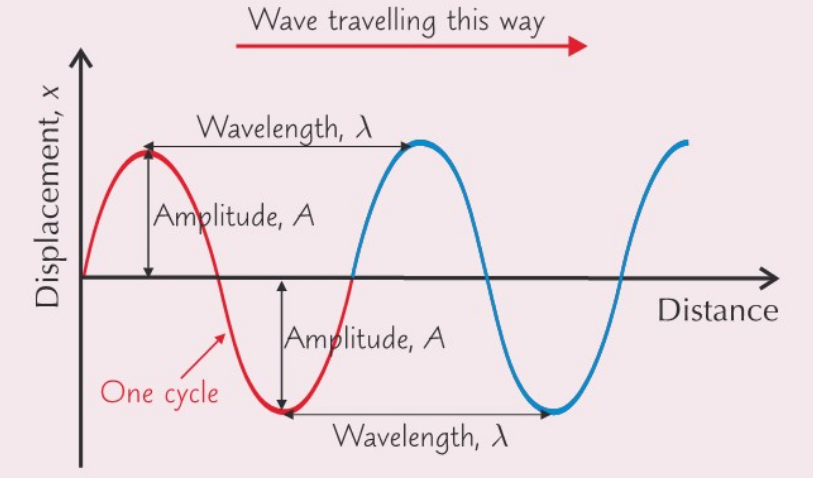
\includegraphics[width=0.7\textwidth]{images/transverseWave.png}
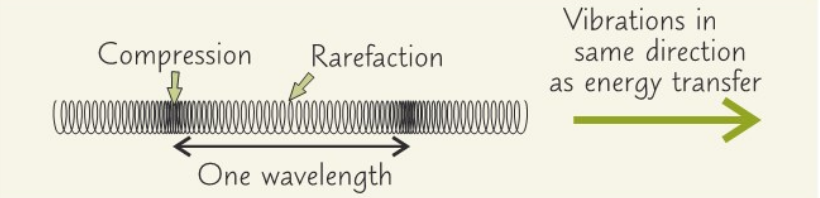
\includegraphics[width=\textwidth]{images/longitudinalWave.png}
\end{center}

\subsection{Interference}

Superposition (Interference) happens when two or more waves pass through each other.

At the moment when waves cross, their displacements add together to form the new wave:

\begin{center}
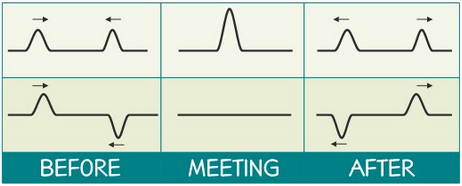
\includegraphics[width=0.5\textwidth]{images/superposition.png}
\end{center}

\subsection{Diffraction}

Diffraction is the spreading out of a wave when a wave travels through a gap or around an object.
All waves can diffract.

The amount of diffraction depends on the wavelength of the wave compared to the size of the gap.

\begin{itemize}
	\item{When the gap is significantly bigger than the wavelength, diffraction is unnoticeable.}
	\item{When the gap is several wavelengths wide, you get noticeable diffraction.}
	\item{When the gap is the same width as the wavelength, you get maximum diffraction.}
	\item{If the gap is smaller than the wavelength, then most of the wave is reflected back.}
\end{itemize}

\subsection{Refractive index}

The refractive index of a material is the ratio of the speed of light in a vacuum divided by the speed of light in the material.

\subsubsection{Snell's Law}

Snell's law relates the refractive index of a two materials to the angle of incidence and angle of refraction:

$$
n_1 \sin{\theta_1} = n_2 \sin{\theta_2}
$$

Here, $\theta_1$ is the angle the ray is from the normal in material 1, and same with $\theta_2$.

\begin{center}
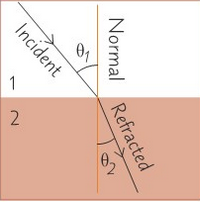
\includegraphics[]{images/incidentAngle.png}
\end{center}

When light moves into a more optically dense material, the light refracts towards the normal, and when light moves into a less optically dense material it refracts away from the normal.

\subsubsection{Critical Angle}

The critical angle ($\theta_c$) is when a ray is diffracted so that the angle of refraction is 90\textdegree from the normal. An angle larger than the critical angle will cause the ray to be reflected back into the material. This is called \textbf{total internal reflection}.

When the angle of refraction is 90\textdegree then:

\begin{align*}
n_1 \sin{\theta_1} &= n_2 \sin{\theta_2} \\
n_1 \sin{\theta_1} &= n_2 \sin{90} = n_2 \\
\sin{\theta_c} &= \frac{n_2}{n_1} \\
\end{align*}

\begin{center}
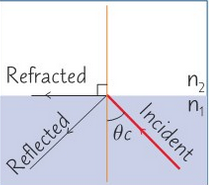
\includegraphics[]{images/criticalAngle.png}
\end{center}

\subsection{Fibre-optics}

Total internal reflection is when the angle of incidence is larger than the critical angle, so the ray gets reflected.

Fibre-optics use this to transport light.

\begin{center}
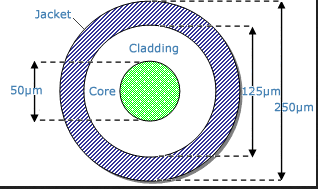
\includegraphics[]{images/opticalFibreCrossSec.png}
\end{center}

The core is made out of a flexible glass/glass polymers. The cladding is made out of a lower refractive index material, so that total internal reflection happens. The jacket is usually for protection and so is usually made out of rubber.

\subsubsection{Absorption}

Some rays in a signal in an optical cable can be absorbed along the way, resulting in a loss of amplitude.

\begin{center}
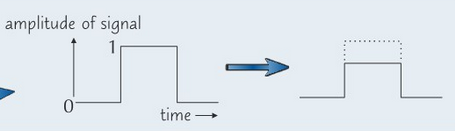
\includegraphics[]{images/opticsAbsorption.png}
\end{center}

\subsubsection{Dispersion}

There are two types of dispersion, but they both lead to the signal becoming broader.

Modal dispersion is when some rays lag behind others, or are ahead of others.

Material dispersion is where different wavelengths in the signal travel at different speeds in the fibre.

Here is the result of both:

\begin{center}

\end{center}

\subsection{Single Slit Diffraction}

When you shine light (or any other wave) through a single slit, and place a screen after the slit, you get a diffraction pattern like this:

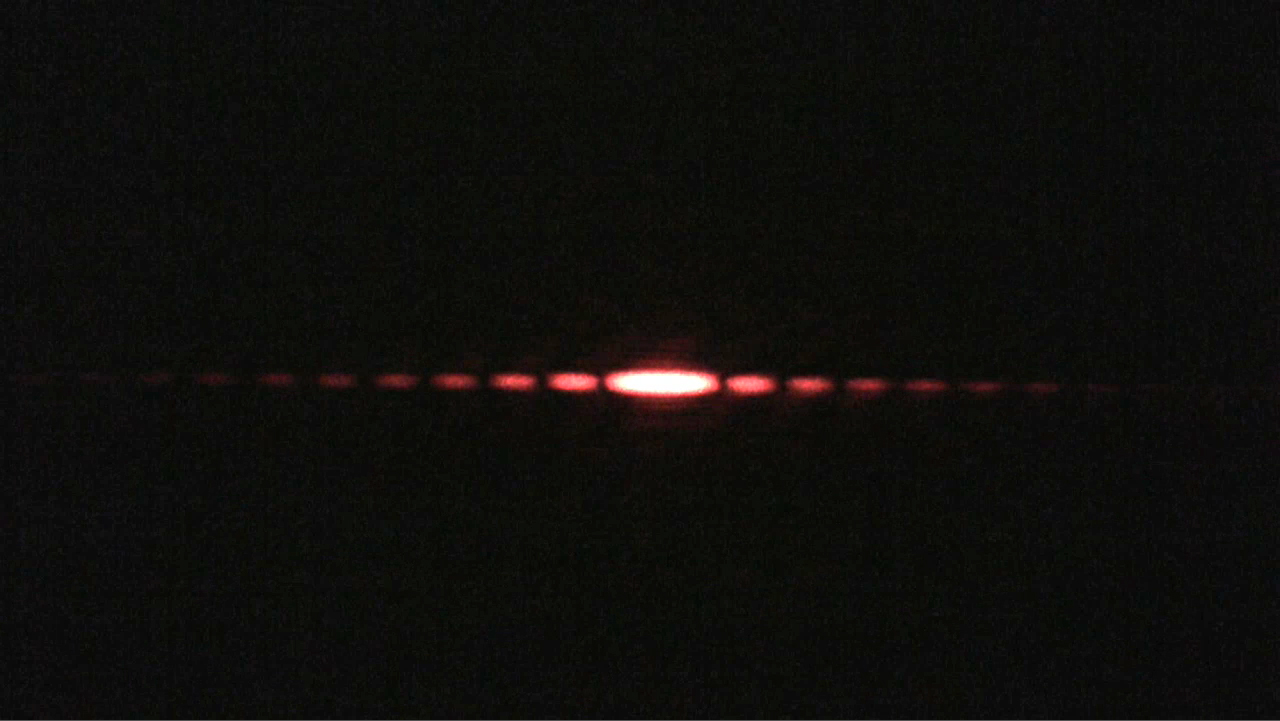
\includegraphics[width=\textwidth]{images/singleSlitDiffPattern.jpg}

To get this clear pattern, you need monochromatic light (all waves from source are same frequency), as if there were light of different wavelengths they would all diffract different amounts.

There is a central bright fringe (the central maximum), with smaller fringes going outwards. These bright and dark fringes are caused by waves in the source interfering (superposing) constructively and destructively. This happens because the source of light is actually a lot of waves all together:

\begin{center}
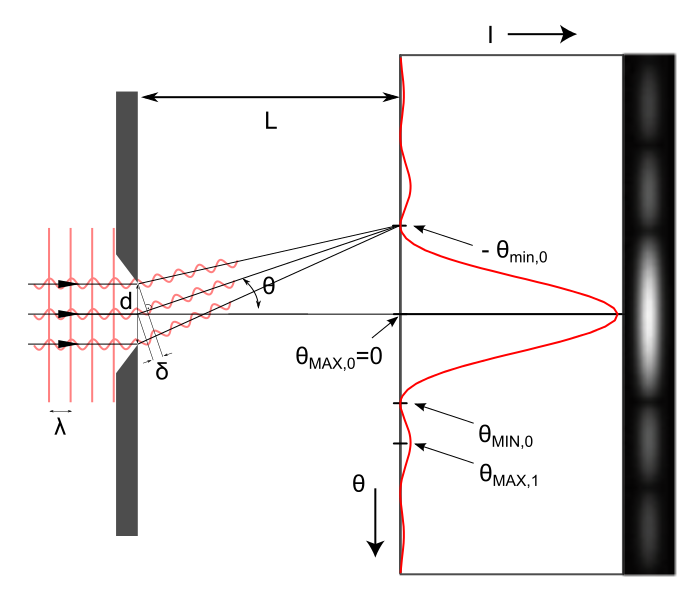
\includegraphics[height=8.5cm]{images/singleSlit.png}
\end{center}

\subsection{Double Slit Diffraction}

Double slit diffraction is very similar to single slit diffraction, however the two slits produce two wave sources that interfere to produce a different pattern. Here is a comparison between the two:

\begin{center}
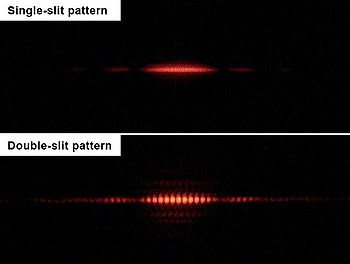
\includegraphics[width=0.6\textwidth]{images/slitDIffCompare.jpg}
\end{center}

The two sources interfere with each other to form bright and dark patches.

Where the waves meet up, they interfere constructively:

\begin{center}
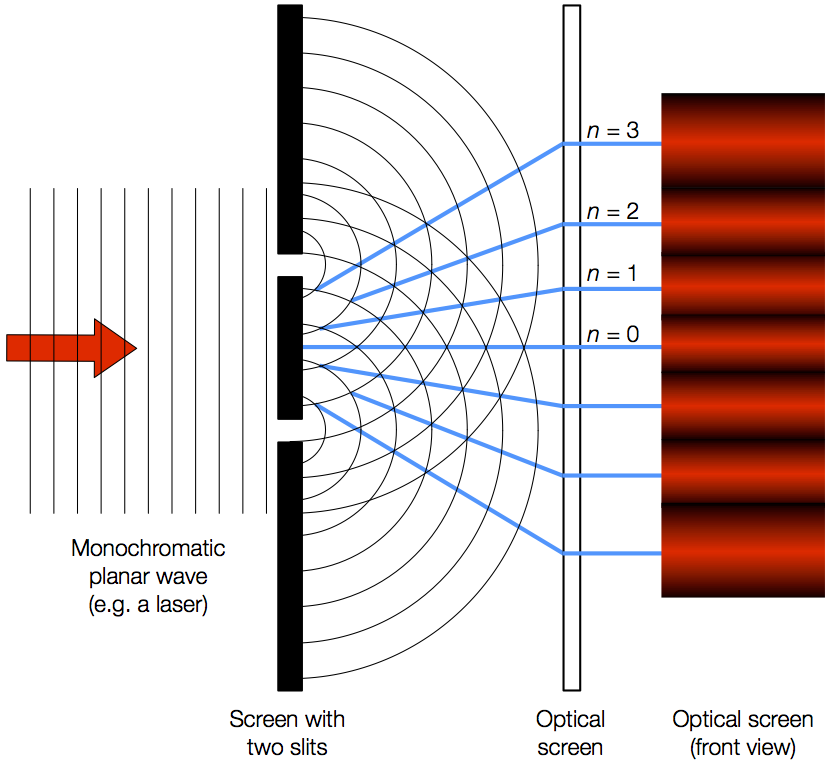
\includegraphics[height=10cm]{images/Double-slit-diffraction-diagram.png}
\end{center}

$n$ is the "order", which is the number of the bright spot from the central maximum. The pattern is mirrored, so so are the order numbers.

The spacing between "fringes" can be found using this equation:

$$
w = \frac{{\lambda}D}{s}
$$

Where $w$ is the fringe spacing, $D$ is the distance of the slits from the screen, and $s$ is the slit spacing. 

Each wave in the light will have to travel different distances depending on where the source of the wave is, and at what angle the wave is travelling in. The difference in distance to travel to each point is called the path difference, measured in wavelengths. When the path difference between waves is a multiple of $\lambda$, then there is constructive interference, producing a bright spot, while at every $\frac{1}{2}$ multiple of $\lambda$, each wave is 180\textdegree out of phase (or $\pi$ radians), so they destructively interfere creating the dark patches.

So at the first order, the path difference would be $\lambda$, second order would be $2{\lambda}$, and so on.

\begin{center}
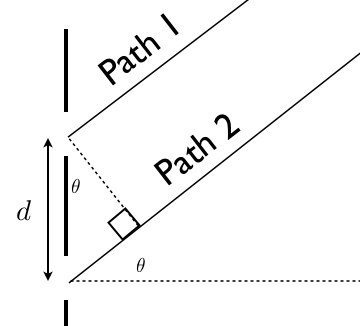
\includegraphics[width=0.5\textwidth]{images/pathDifference.jpg}
\end{center}

To find the angle of the light leaving the slits at a bright spot (an order), you can use this formula:

$$
n\lambda = d\sin\theta
$$

Where $n$ is the order, $\lambda$ is the wavelength and $d$ is the distance between slits. The path difference is the extra part of the line in Path 2.

$n{\lambda}$ can be replaced with the path difference, as this is the opposite side of the triangle in the above image, where $d$ is the hypotenuse. So in theory, this equation can be used to find the slit spacing/angle at any path difference as long as you know what that path difference is.

When doing any slit experiment with white light, the spectrum will separate, with blues towards the middle, and reds going out:

\begin{center}
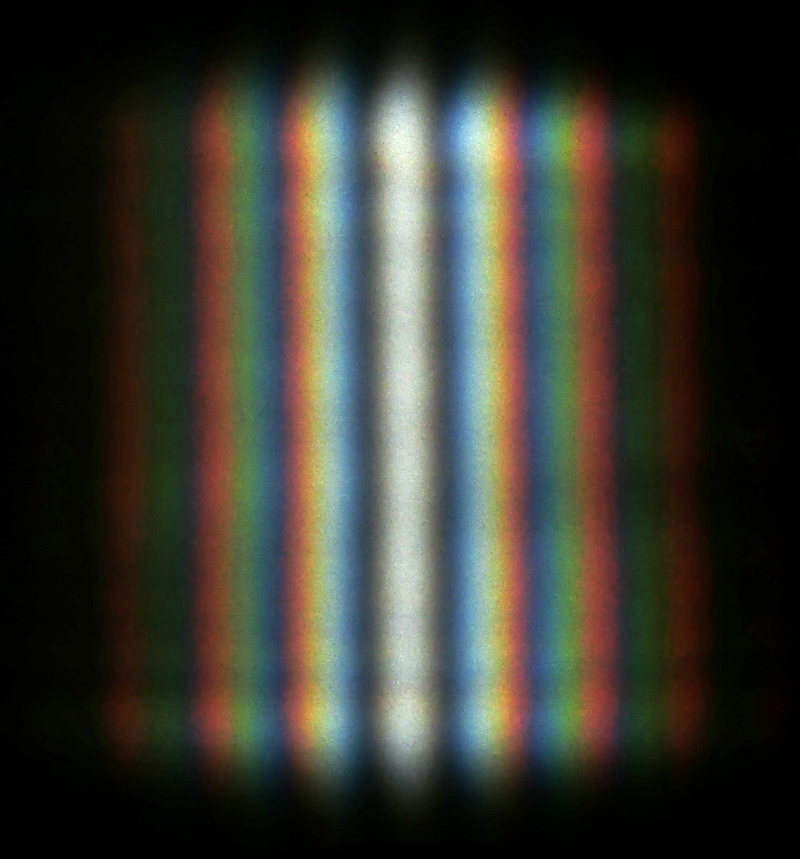
\includegraphics[height=6cm]{images/doubleSlitWhite.png}
\end{center}

\subsection{Diffraction Gratings}

Diffraction gratings work almost the same as the double slit experiment, however the slit spacing is usually very small. When you add more than two slits, the pattern seen has brighter and narrower fringes, and darker dark-fringes. A diffraction grating has many many small slits, so the pattern is very sharp.

Usually in a question you will be given the number of slits/lines in a diffraction grating per millimetre or something. To convert this to the distance between slits, you need to do:

$$
d = \frac{measurment}{lines \, per \, measurement}
$$

For example, if you have 500 lines/millimetre, then to convert this you do:

$$
\frac{10^{-3}}{500} = 2 \times 10^{-6}
$$

This is the $d$ distance to use in the equation in the last section.

\subsection{Polarisation}

Polarisation is where you take a bunch of waves all oscillating in different planes, and filter it so that you are left with all waves oscillating in the same plane.

This only works for transverse waves and does not work with longitudinal waves, since they do not oscillate on different planes, as their oscillation will always be in the direction of travel.

Here is a diagram showing polarisation:

\includegraphics[width=\textwidth]{images/polarisation.png}

If you use two filters at a 90{\textdegree} angle to each other, then all waves will be blocked, since this pretty much becomes a small dot for the wave to get through (if you an imagine having the two slits together), so all up and down movement will be blocked.

Polarisation is used as evidence to show that EM waves are transverse.

TV and radio signals are polarised based on the orientation of the rods on the broadcasting aerial. With TV receiving aerials, you need to orient the aerial so that it is in line with the incoming waves.

\subsubsection{Polarising Glasses}

Polarising sunglasses are used to reduce glare from light reflected off of objects. This is because when light is reflected, it is polarised. Polarising glasses contain a filter to block this light.

\subsection{Standing Waves}

Standing/Stationary waves is the superposition of two progressive waves with the same frequency moving in opposite directions.

Standing waves are waves that do not transfer energy in any direction, however they do still oscillate.

One way of creating standing waves is by having a driving oscillator at one end of a stretched string, with the other end fixed. When the oscillator is on, the waves created are reflected backwards, and superpose. If the wavelength the oscillator is producing is in the sequence $\frac{1}{2} l$, where $l$ is the length of string, then it will form a standing wave.

\subsubsection{Harmonics}

As talked about above, at certain wavelengths, stationary waves are formed on a string.
These are the harmonics. Nodes form where the wave does not seem to oscillate (the two opposing waves cancel out at this point), and anti-nodes are where the standing wave oscillates the most.

The first harmonic looks like this:

\begin{center}
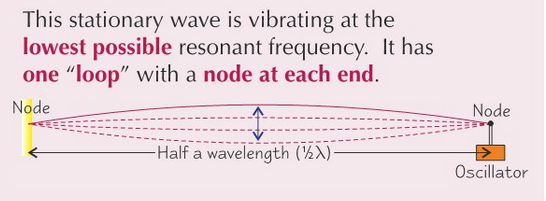
\includegraphics[width=0.7\textwidth]{images/firstHarmonic.png}
\end{center}

The first harmonic has two nodes, one at each end, and one anti-node in the middle.

Nodes are usually marked with a dot, and anti-nodes with a cross.

Here is the second harmonic:

\begin{center}
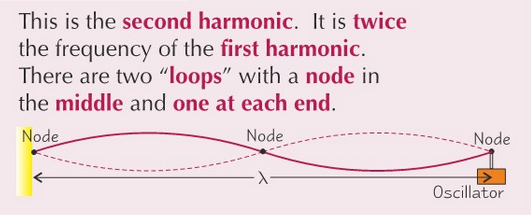
\includegraphics[width=0.7\textwidth]{images/secondHarmonic.png}
\end{center}

For the first harmonic on a string, you can use this equation to find the frequency:

$$
f = \frac{1}{2l} \sqrt{\frac{T}{\mu}}
$$

Where $\mu$ is the mass per unit length of the string, $T$ is the tension in the string, and $l$ is the length of the string.

\subsection{Sound}

Stationary waves can also be created in air too. This is how clarinets and trumpets work. A wave is formed in the tube of the instrument, and is reflected by an area of high/low pressure (formed by the wave itself) at the end of the tube. Opening holes in the tube creates an opening closer to the mouthpiece, creating shorter wavelengths. This only produces odd numbered harmonics, since a node/anti-node is needed at the end to reflect the wave:

\begin{center}
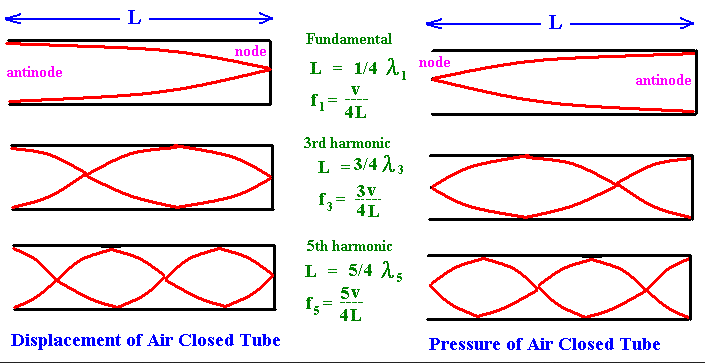
\includegraphics[width=\textwidth]{images/harmonicInTube.png}
\end{center}

\newpage
\section{Mechanics And Materials}

\subsection{Vectors}

\subsection{Moments}

\subsection{Centre of Mass}

\subsection{Newton's Laws}

\subsection{SUVAT}

\subsection{Collisions}

\subsection{Work Done}

\subsection{Hooke's Law}

\subsection{Stress and Strain}

\subsection{Young's Modulus}


\newpage
\section{Electricity}

\subsection{Voltage, Current and Resistance (Ohm's law)}

\subsubsection{Voltage and E.M.F}

Voltage is the amount of enegry provided (electric potential energy) per unit charge, or \textbf{work done per unit charge.}

E.M.F (Electromotive force) is the voltage supplied by a cell/power source with no resistance (even no internal resistance).

\subsubsection{Current}

Current is the rate of flow of charge (Coulombs per second).

$$
I = \frac{\Delta Q}{\Delta t}
$$

\subsubsection{Resistance}

When you create a potential difference across a component, a current will flow. The amount of current that makes it through the component depends on the resistance of the component.

$$
R = \frac{I}{V}
$$

Measured in Ohms ($\Omega$).

\subsubsection{Ohm's Law}

For ohmic conductors, if physical conditions are kept constant (such as temperature), $I \propto V$.

The constant of proportionality is actually the resistance.

$$
V = IR
$$

\subsection{IV Graphs, Diodes and Thermistors}

IV graphs (or current voltage graphs) show the characteristics of a conductor.

\subsubsection{Ohmic Conductor IV}

If given an IV graph for an ohmic conductor, then it will be a straight line where the gradient is $\frac{1}{R}$, since $I$ is on the $y$ axis rather than the $x$ axis ($y = mx + c \rightarrow I = \frac{1}{R}V$).

\begin{center}
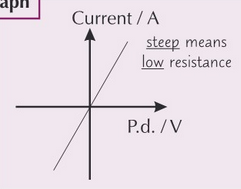
\includegraphics[]{images/ohmicCond.png}
\end{center}

\subsubsection{Filament Lamp IV}

A filament lamp however, is not an ohmic conductor. The resistance of the filament in the bulb increases as the temperature of the filament increases, which is due to the voltage.

\begin{center}
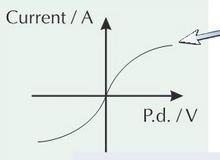
\includegraphics[]{images/bulbIV.png}
\end{center}

\subsubsection{Diodes}

A diode is a component that only lets current flow in one direction. The forward bias is the direction the current is allowed to flow. If current flows in reverse bias, it will be blocked, unless it is above like 1000V or whatever rating is for the diode, and at this point the diode breaks. 

Most diodes require a threshold voltage (in forward bias) before current starts to flow. This is usually around 0.6V.

\begin{center}
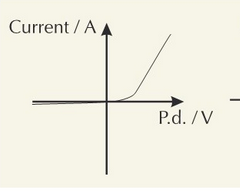
\includegraphics[]{images/diodeIV.png}
\end{center}

\subsubsection{Thermistors}

The resistance of a thermistor depends on the temperature. We only need to know about NTC thermistors - Negative Temperature Coefficient.

\begin{center}
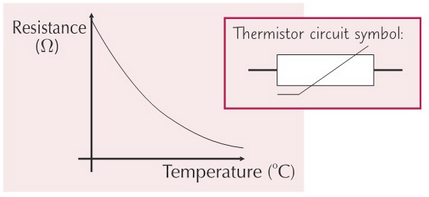
\includegraphics[]{images/thermistor.png}
\end{center}

IV graph for thermistor:

\begin{center}
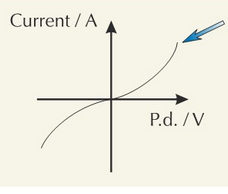
\includegraphics[]{images/thermistorIV.png}
\end{center}

\subsection{Resistivity}

\newpage
\section{Circular, Periodic and Harmonic Motion}

\newpage
\section{Thermal Physics}

\newpage
\section{Fields}

\newpage
\section{Nuclear}

\newpage
\section{Astrophysics}

\subsection{Lenses}

To understand telescopes, you need to understand lenses.

Lenses work by refracting light to produce the effect you want. Converging lenses bring the light rays together, whereas diverging lenses separate the rays further apart.

Every lens has a focal point. The focal point is the point every ray refracted has to pass through. For divergent lenses, they will never pass through the focal point (unless it goes straight through the middle), so the extension of the rays backwards have to pass through the focal point in front of the lens.

When drawing lens diagrams you have to draw a ray going from the object and straight through the middle of the lens, and one that goes horizontally from the image, through the lens and through the focal point (called the principle focus).

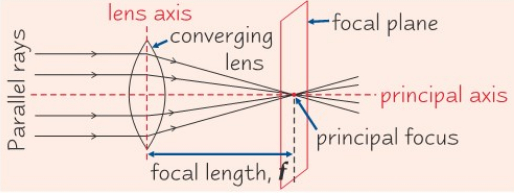
\includegraphics[width=\textwidth]{images/lensDiagram.png}

The image produced by a lens can either be real or virtual. A real image is made up of the actual rays, and can be projected onto a screen. A virtual image is when the rays do not actually produce an image, but instead your eye traces the rays back to form an image.

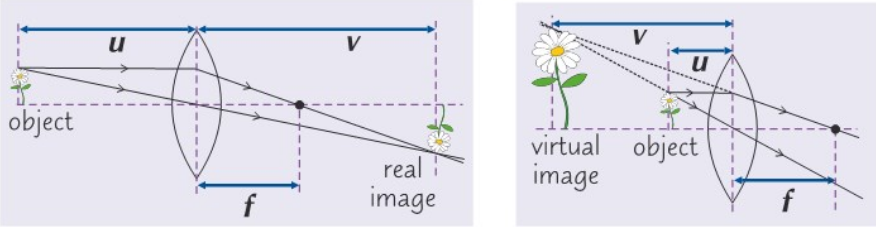
\includegraphics[width=\textwidth]{images/realAndImaginaryImages.png}

$u$ is the distance of the object from the lens, while $v$ is the distance of the image from the lens, and $f$ is the focal length.

You can find the focal length from the equation:

$$
\frac{1}{u} + \frac{1}{v} = \frac{1}{f}
$$

The magnification of a lens is:

$$
\frac{h_i}{h_o} = -\frac{v}{u}
$$

Where $h_i$ is the height of the image, and $h_o$ is the height of the object. The negative sign on the second part is due to the image being flipped. If you think about it, $h_i$ would also be negative if the image is flipped, since the image would be upside down.

Just a side note $\Rightarrow$ $2f$ is the radius of the (imaginary) sphere used to make the lens.

\subsection{Refracting Telescope}

A refracting telescope uses two converging lenses:

\begin{enumerate}
	\item{
		\textbf{Objective lens} - Gathers as much light as possible from the source, and converges the rays from the source to produce an image.
	}
	\item{
		\textbf{Eye lens} - Acts as a magnifying glass on the real image to produce a magnified virtual image.
	}
\end{enumerate}

If you assume the object you are looking at is at infinity, then all rays from it are parallel, and the real image is formed on the focal plane. Rays that are not parallel would be converge somewhere else on the focal plane.

A telescope is set up so that the principal focus (focal point) of the lens is in the same position as the principal focus of the eye lens, so that the final magnified image appears to be at infinity.

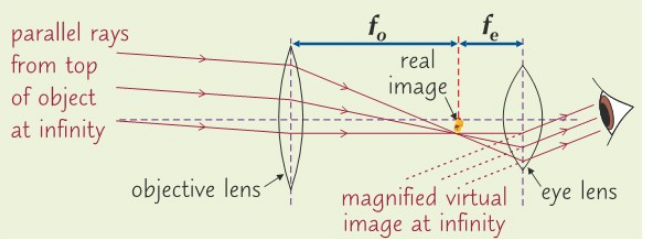
\includegraphics[width=\textwidth]{images/refactingTeleLayout.png}

To find the magnification of a telescope, you take the angle subtended (angle from top to bottom of object) by the image, and divide it by the angle subtended by the object:

Subtending:

\begin{center}
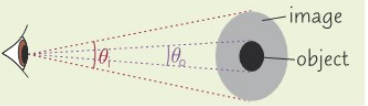
\includegraphics[width=0.5\textwidth]{images/subtend.png}
\end{center}

Equation:

$$
M = \frac{\theta_i}{\theta_o}
$$

This can also be done in terms of focal length, where $f_o$ is the objective lens, and $f_e$ is the eye lens:

$$
M = \frac{f_o}{f_e}
$$

$f_o$ will be much bigger than $f_e$ since telescopes are used to magnify.

\subsection{Reflecting Telescope}

Reflecting telescopes use two mirrors and a converging lens:

\begin{enumerate}
	\item \textbf{Primary Mirror} - A parabolic concave mirror at the back of the telescope.
	\item \textbf{Secondary Mirror} - A convex secondary mirror near the front of the telescope.
	\item \textbf{Eye Lens} - Same purpose as on the refactor telescope.
\end{enumerate}

The principle focus of the primary mirror is in front of the mirror, so to view the image without blocking the light, the image is reflected by the secondary mirror, and this mirror also decreases the angle of the light from the horizontal due to it's convex shape, so the light will focus past the mirror, and then be lined up again after the focal point by the eye lens.

This secondary mirror can also be flat if the light's angle does not need to be changed.

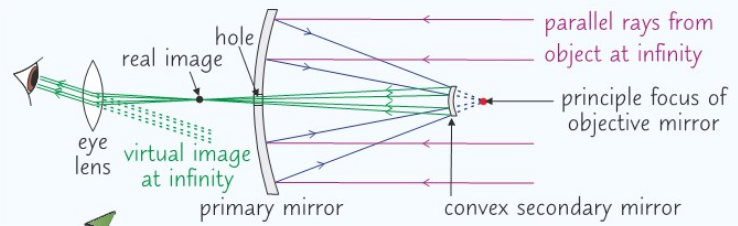
\includegraphics[width=\textwidth]{images/reflectingTele.png}

Pretty much just nicking CGP images (but that is because they are decent).

\subsection{Resolving Power of a Telescope}

The resolving power of a telescope is the measure of how much detail you can see through the telescope.

It is dependant on the minimum angle that the telescope can distinguish two points at. The smaller the angle, the better the telescope can distinguish two points close together.

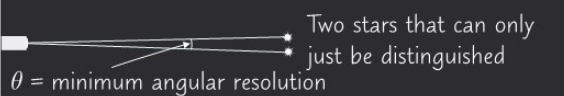
\includegraphics[width=\textwidth]{images/angularResolution.png}

The minimum angle is limited by diffraction. If the light passes through a circular aperture (tube of telescope), then it will diffract and form a pattern like the single slit experiment, however in 2 dimensions. The central maximum of that pattern is called the "Airy disc". Two light sources can just about be distinguished if one of the sources' Airy discs is at least as far away as the first minimum of the diffraction pattern formed by the other star (first dark band going out from middle).

\begin{center}
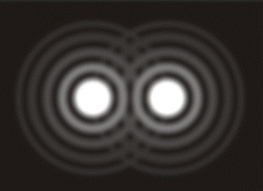
\includegraphics[width=5cm]{images/airyDisc.png}
\end{center}

This leads to the Rayleigh criterion:

$$
\theta \approx \frac{\lambda}{D}
$$

Where in our case, $D$ is the diameter of the objective lens/mirror. The larger the mirror/lens, the less diffraction will happen, therefore there will be a clearer image.

\subsection{Problems with Refracting Telescopes}

\begin{itemize}
	\item Glass refracts light of different wavelengths different amounts, so the different colours of light from an object will not all focus onto the focal plane of each lens. Causes chromatic aberration (where each colour forms a different image).

	\item Bubbles and impurities in the glass block some light from the source, and making large lenses that are of good quality are expensive and difficult to make.

	\item Large lenses are very heavy compared to mirrors.

	\item For large magnification, the objective lens needs to have a very long focal length, so the barrel of a large refracting telescope would be huge, and very expensive due to the building needed to house it.
\end{itemize}

\subsection{Problem with Reflecting Telescopes}

If the mirror is not a perfect parabolic shape, then not all rays reflected by the mirror will meet at the focal point exactly, creating a blurry image. This is called spherical aberration.

\begin{center}
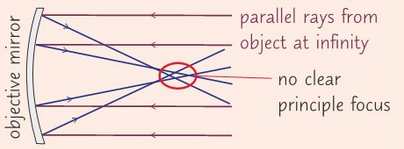
\includegraphics[width=0.7\textwidth]{images/sphericalAbb.png}
\end{center}

\subsection{CCD's (Charge-Coupled Devices)}

CCD's are camera sensors.

CCD's are silicon chips roughly the size of a postage stamp, with grids of pixels. Each square on the grid detects photons.

When a photon hits a pixel in the grid, they cause electrons to be released (photoelectric effect), which changes the charge on the pixel, and the charge on each pixel can be used to create a digital signal.

This signal tells the firmware (in the CCD unit somewhere) the intensity of light at that pixel, so from this an image can be formed.

\subsubsection{Comparing the human eye to a CCD}

\begin{itemize}
	\item The eye can only detect visible light, whereas a CCD can detect infrared, visible and UV light.

	\item CCD's are better for capturing fine detail, since the eye's spacial resolution (distance between objects so that they become distinguishable) is higher (worse) at 100 $\mu$m, whereas a CCD usually has a spacial resolution of 10 $\mu$m.

	\item Quantum efficiency is 80\% higher for CCD's compared to the eye. The quantum efficiency is the proportion of incident photons detected. For the eye, this is around 1\%.

	\item The human eye doesn't need more equipment (hopefully), and looking down a telescope is easier than setting up a whole CCD.

	\item When using a CCD you can keep the images and share them globally if you want.
\end{itemize}


\subsection{Radio Telescopes}

Radio telescopes work very similarly to reflecting telescopes, where you have a parabolic dish that collects light, and reflects it towards the middle.

A radio telescope does not need an equivalent to an eye lens, the radio waves are instead reflected onto a pre-amplifier, which then goes onto the antenna, where it is turned into a digital signal.

Radio telescopes are usually manoeuvrable, so they can track the radio source.

\begin{center}
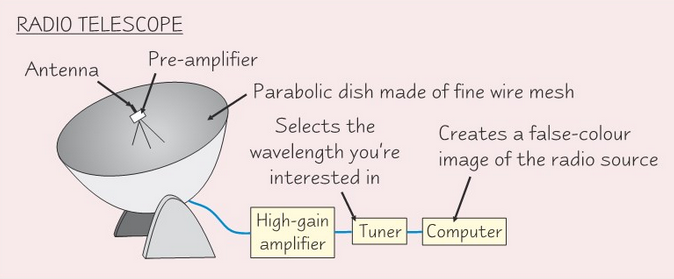
\includegraphics[width=\textwidth]{images/radioTelescope.png}
\end{center}

Radio waves have much longer wavelengths ($\times 10^6$ longer). This means that the resolving power of a radio telescope will be much lower than a reflecting telescope, due to the Rayleigh criterion: $\theta = \frac{\lambda}{D}$. The dish would have to be the size of the UK to get a resolving power the same as an optical telescope.

To get around this, we link a bunch or radio telescopes together (makes an equivalent to one huge dish the size of the separation of the telescopes), and using some algorithms you can combine all the signals to produce one image. This can make the resolving power thousands of times better than an optical telescope.

The longer wavelength of radio waves also means that irregularities in the reflecting surface do not have as much of an effect, since the gaps are much smaller than the wavelength.

This means that we can just use wire mesh to reflect the waves, as this is less expensive and easier to make. Also, the maximum gap allowed on the dish is $\frac{\lambda}{20}$ (for all telescopes) to prevent spherical aberration, so less precision needed.

Radio telescopes have to scan across the object to form an image.

\subsection{Problems with telescopes on the ground.}

The main problem for telescopes on the ground is the atmosphere. The atmosphere only lets certain wavelengths through. Light in the visible spectrum is mostly let through, so optical telescopes are fine on the surface.

\subsection {Arcseconds}

Arcseconds are a unit of measuring angles. They are used for measuring angular distances in the sky. Arcseconds are used rather than degrees because usually the angular distance between objects in the sky are very small, so a smaller unit of measurement than the degree was needed.

They have nothing to do with time, it's just because the Babylonians decided to use the same format as time for their astronomical angles.

$$
1 \, arcsecond = \frac{1}{3600} \, degrees
$$

$$
1 \, arcminute = \frac{1}{60} \, degrees
$$

and so on.

\subsection{Astronomical Units}

The astronomical unit ($AU$) is the average distance between the centre of the Sun and the centre of the Earth.

\subsection{Parsecs}

Full definition: 1 parsec is the distance to a star which subtends an angle of 1 arcsecond to the line from the centre of the Earth to the centre of the Sun.

Parallax is when you look out of the car window and stuff that is closer seems to move faster than things that are far away. The angle of parallax (stellar parallax) in this case, is the angle between the centre of the Sun, the object, and the centre of the Earth.

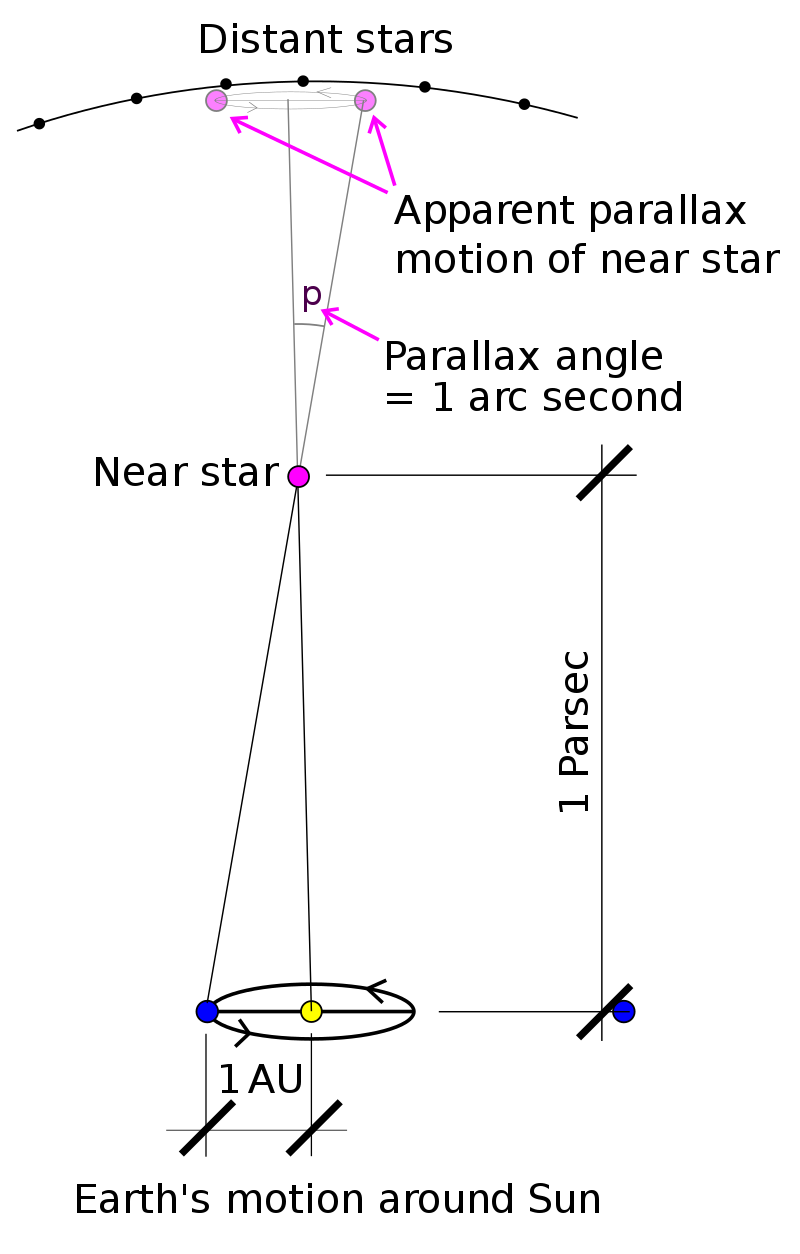
\includegraphics[width=\textwidth]{images/parsec.png}

The parsec is used because it is very easy to get the distance in parsecs when given the parallax angle.

$$
d = \frac{1}{\theta}
$$

This works because $\theta$ is usually a very small angle (arcseconds are tiny), so we can use the small angle approximations. $\tan{\theta} \approx \theta$

The distance to the object is the adjacent, the opposite is 1 $AU$, and so

\begin{align*}
	\tan{\theta} &= \frac{o}{a} \\
	\tan{\theta} & \approx \theta \\
	\theta &= \frac{o}{a} = \frac{1}{d} \\
	d &= \frac{1}{\theta}
\end{align*}

\subsection{Light-Years}

1 light-year is the distance light travels in 1 year in a vacuum ($\approx 3 \times 10^8 \, m$).

Light-years are useful because they help you understand how hugely far away stuff is. For example, when you look at the Moon, light takes 1 second to come from the Moon (reflected off of the surface), so when you look at the moon you are looking at it as it was 1 second ago. Or if a galaxy is 10 light-years away, then you are looking at it as it was 10 years ago.

\subsection{Magnitude of Stars}

The magnitude of a star is a rating system for comparing the brightness of stars, compared to the star Vega (magnitude of 0).

The scale goes:

\begin{itemize}
	\item \textbf{0} - Magnitude of the star Vega.
	\item \textbf{6} - Dimmest star visible to the human eye.
\end{itemize}

There is apparent magnitude, and absolute magnitude.

Apparent magnitude is the magnitude of the star as looking at it in the night sky, while absolute magnitude is what the apparent magnitude would be if the star was \textbf{10 parsecs} away.

\textbf{The scale is infinite} however. For example, the Sun has an apparent magnitude of -26.7. Absolute magnitude is useful for comparing close stars, like the Sun, with other stars. The Sun's absolute magnitude is 4.84.

The equation for finding absolute and apparent magnitude is:

$$
m - M = 5 \log \left({\frac{d}{10}}\right)
$$

Where $m$ is the apparent magnitude, $M$ is the absolute magnitude and $d$ is the distance to the star in parsecs.



\subsection{Black Bodies and Power Output of Stars}

\textbf{A black body is a body that absorbs and radiates all incident radiation wavelengths.} Black bodies have a peak wavelength that it emits, based on the temperature of the body.

\subsubsection{Wein's Displacement Law}

A star can be approximated as a black body. As a star gets hotter, it tends to become more blue:

\begin{center}
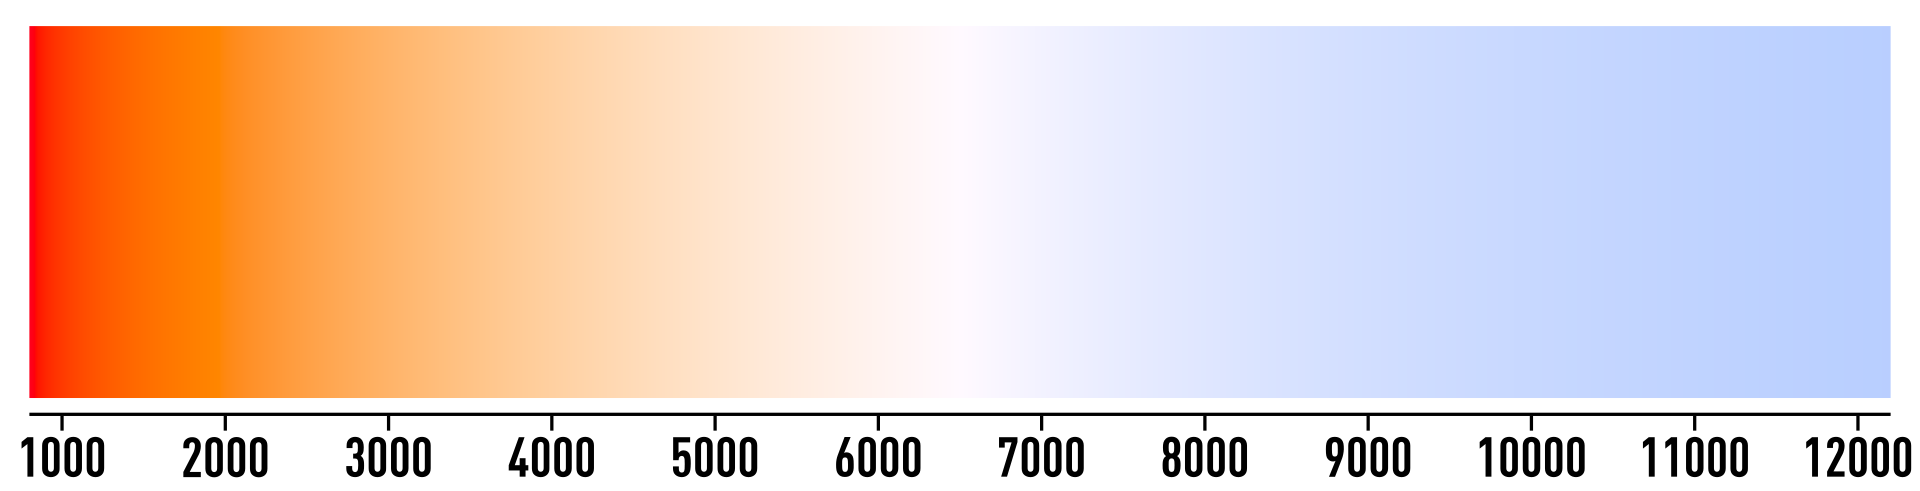
\includegraphics[width=\textwidth]{images/blackBodyColour.png}
\end{center}

Stars of different temperatures have a different peak wavelength:

\begin{center}
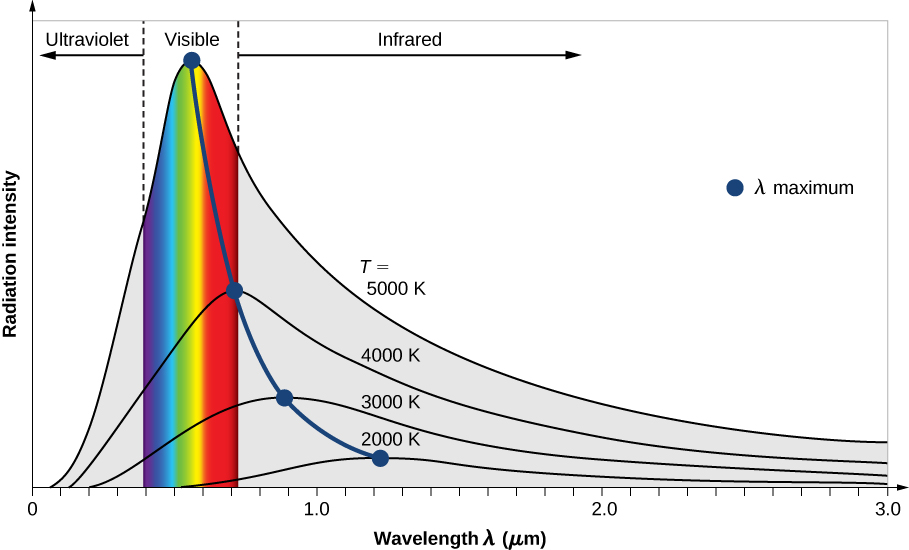
\includegraphics[width=\textwidth]{images/blackBodyPeakWav.jpg}
\end{center}

The $\lambda$ at peak intensity is inversely proportional to the absolute temperature:

$$
\lambda \propto \frac{1}{T}
$$

So $\lambda_{\text{max}} T =$ constant.

That constant is $2.9 \times 10^{-3}$.

\subsubsection{Stefan's Law}

Stefan's law is used to find the power output of a black body:

$$
P = {\sigma}AT^4
$$

Where $\sigma$ is Stefan's constant, $A$ is the area of the body, and $T$ is the absolute temperature of the body (in kelvin).

\subsubsection{Side Note:}

If (and only if) two stars have the same absolute magnitude, they have the same power output, since stars with the same absolute magnitude will produce the same amount of visible light, so they will either be very similar, or have higher temperature but lower surface area, or visa versa.

\begin{align*}
P_1 &= P_2 \\
\sigma A_1 T^4_1 &= \sigma A_2 T^4_2 \\
A_1 T^4_1 &= A_2 T^4_2 \\
\frac{A_1}{A_2} &= \frac{T^4_2}{T^4_1}
\end{align*}

\subsubsection{Brightness Difference.}

To find the brightness difference between two stars, you do:

$$
2.51^{m_1 - m_2}
$$

Where $m_x$ is the apparent magnitude.

This works because the magnitude scale (for stars) is logarithmic (however the scale goes backwards so it seems like an exponential), so a difference of 1 in magnitude is a difference of $100^{\frac{1}{5}} = 2.51$ times brighter/dimmer each step.

\subsection{Classification of Stars}

Stars are not only classified by their absolute magnitude, but also but their spectral class.

The spectral class of a star is determined by it's temperature, and it's spectral absorption lines.

The spectral classes go:

O, B, A, F, G, K, M

Oh Be A Fine Girl Kiss Me (Acronym)

Unfortunately, this table has to be remembered:

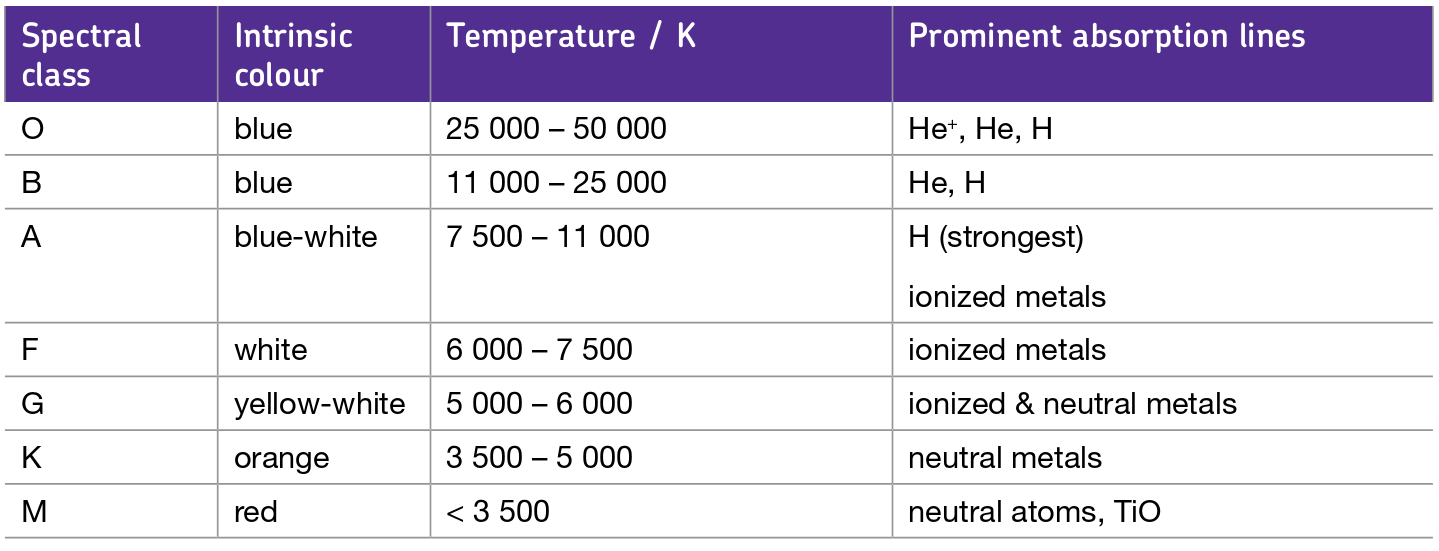
\includegraphics[width=\textwidth]{images/spectralClasses.png}

Originally, stars were only classified based on their hydrogen alpha ($H \alpha$) absorption line (656.28 nm). The hydrogen alpha line is only formed when an electron in a hydrogen atom is excited from level 2 to level 3, absorbing a photon. \textbf{The photon is usually produced by the core of the star, and is absorbed by the atmosphere of the star, then emitted in a random direction}, so the light of that wavelength will no longer travel towards Earth, which is why the line is visible. In reality, the line is only slightly fainter than the other wavelengths, since it is emitted again, but in a random direction.a

Steps in order:

\begin{enumerate}
\item \textbf{Electron in hydrogen atom in atmosphere is in n = 2 state.}
\item \textbf{Light passing through excites that electron to n = 3.}
\item \textbf{The electron de-excites. This emits an electron in a random direction.} The electron has to drop back down to n = 2 for us to see it though, since if it drops to n = 1, then it will be UV and will be blocked by the atmosphere.
\end{enumerate}

\begin{center}
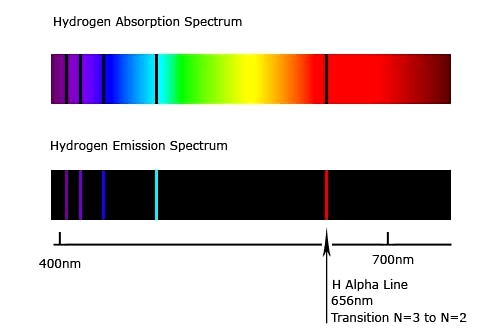
\includegraphics[width=0.6\textwidth]{images/hydrogenAlpha.jpg}
\end{center}

This isn't a good way of doing it since if a star is very hot, the hydrogen is ionised, so it cannot be excited, likewise, if the star is too cold, then it cannot produce enough energy to excite the hydrogen, so it is a goldilocks scenario.

In the old system, A was the strongest $H \alpha$ line, and O was the weakest (alphabetical order).

\subsubsection{Hertzsprung-Russel Diagram}

The Hertzsprung-Russel diagram plots absolute magnitude of stars in the sky against their temperature (or spectral class).

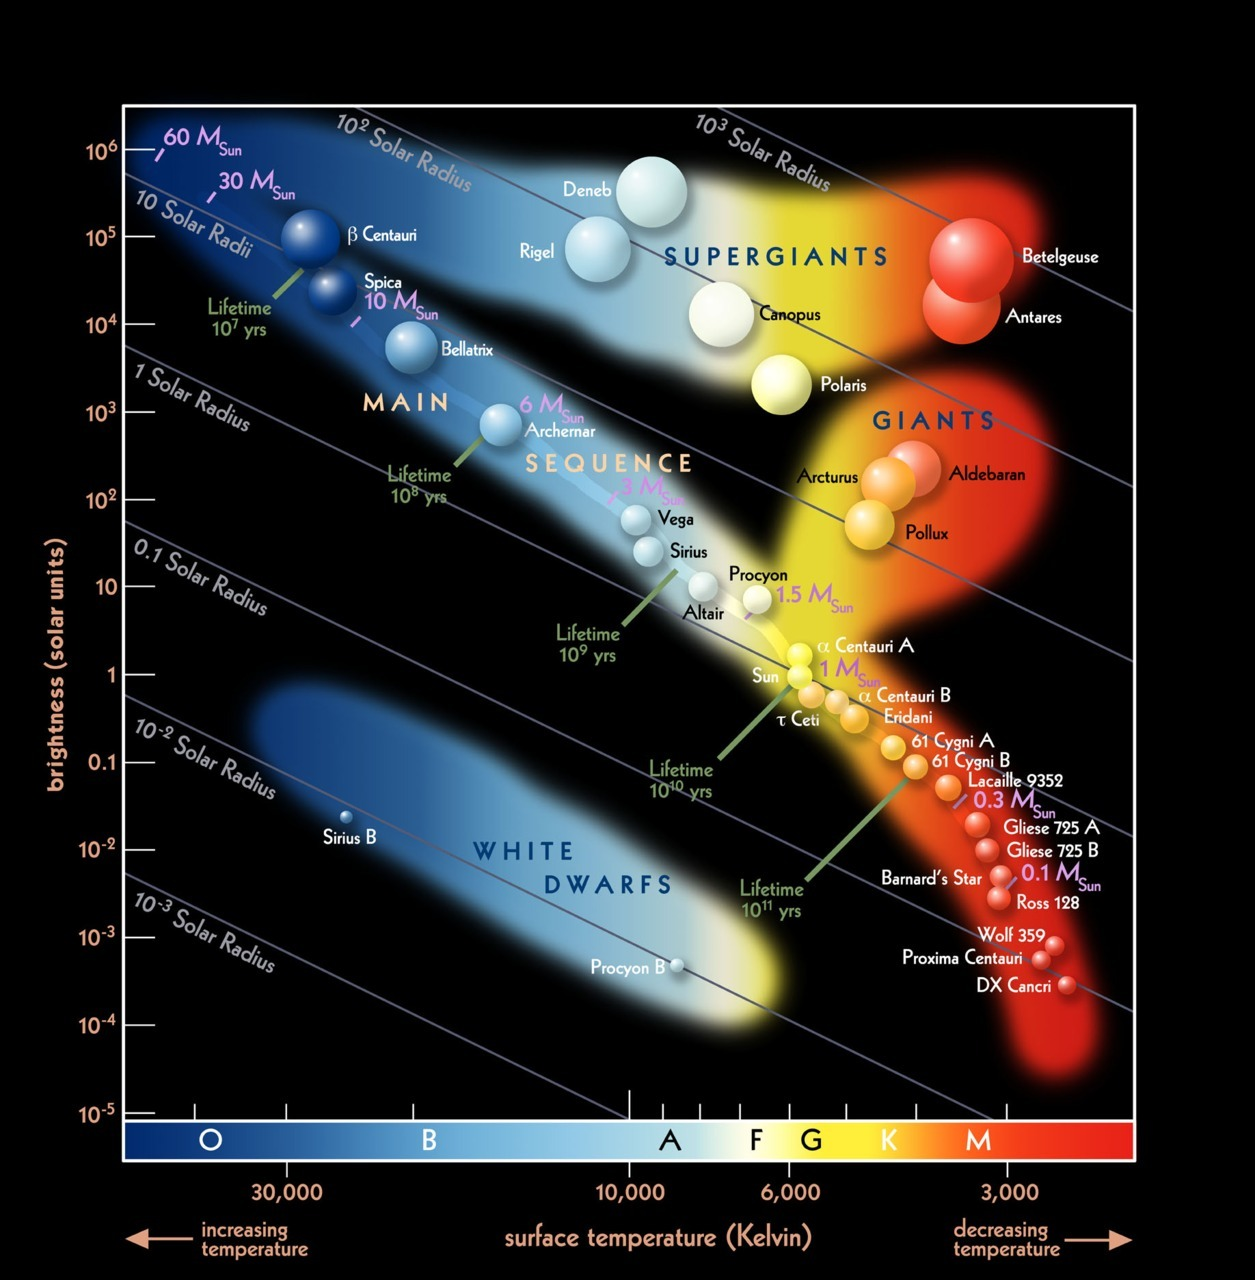
\includegraphics[width=\textwidth]{images/hertzsprungRussel.jpg}

The scale's are logarithmic, otherwise the graph would be huge. For A-Level, you have to know the rough area for dwarfs and giants, and what the main sequence line looks like.

The absolute magnitude is on the y-axis (in this case it is in solar units) and ranges from 10 to -15, where -15 is higher on the y-axis. The temperature is on the x-axis, and goes backwards and is logarithmic.

\subsection{Evolution of Stars}

There are two forces in balance in a star. The \textbf{gravitational force} and the \textbf{radiation pressure}. The radiation pressure is the pressure generated by fusion in the core.

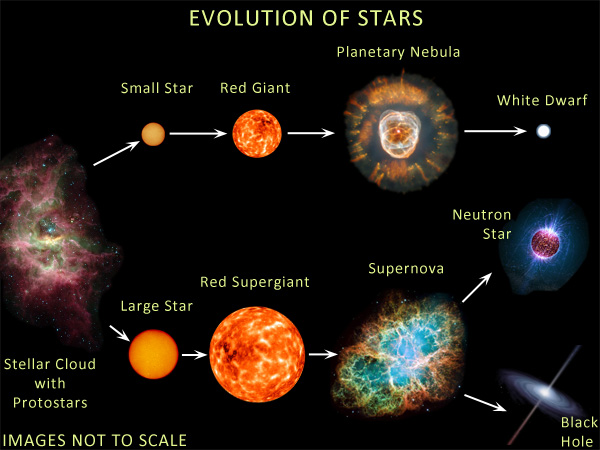
\includegraphics[width=\textwidth]{images/starLifeCycle.jpg}

\subsubsection{All Stars}

Step by step process:

\begin{enumerate}
	\item \textbf{Nebula} - Large gas clouds.

	\item \textbf{Protostar} - Collection of gas pulled together by gravity (similar to gas planet), but does not have enough pressure to start fusion.

	\item \textbf{Main Sequence Star} - Fusion starts when there is enough gravity to create enough pressure for fusion. The GPE $\rightarrow$ KE in the gas as the gas cloud increases mass (ideal gas laws), which increases the temperature of the gas. Fusing Hydrogen into Helium.

	\item \textbf{Depletes Hydrogen} - Gravity becomes stronger than the radiation pressure, so gravity compresses the gas further (GPE $\rightarrow$ KE), so fusion of Helium starts, increasing radiation pressure. The radiation pressure from fusing Helium is greater than Hydrogen, so the star expands and cools.
\end{enumerate}

This is the point where big and small stars are different.

\subsubsection{Small Stars ($< 3$ Solar Masses)}

\begin{enumerate}
	\setcounter{enumi}{5}

	\item \textbf{Red Giant stage} - Since the star has expanded, it is larger, and it has cooled so the colour of the star becomes more reddish.

	\item \textbf{Iron is formed in the core} - Iron requires energy to fuse, so fusion stops here. As more iron is produced in the core, the rate of fusion decreases, until fusion stops.

	\item \textbf{White Dwarf} - Once fusion stops, the outer layers of the star break off, leaving the hot dense core. The core then slowly cools over billions of years into a \textbf{black dwarf} (not enough energy to emit light). Electron degeneracy (EM repulsion) prevents the core from collapsing due to gravity.
\end{enumerate}

\subsubsection{Large Stars ($> 3$ Solar Masses)}

\begin{enumerate}
	\setcounter{enumi}{5}

	\item \textbf{Red Supergiant stage} - The star has expanded to a huge reddish star due to the expansion.

	\item \textbf{Iron is formed in the core} - Same process as in small stars.

	\item \textbf{Supernova} - Gravity compresses the star due to fusion stopping. This causes the core to collapse, and when it rebounds, it causes a supernova explosion that ejects all of the layers off of the star. This explosion also causes the fusion of heavier elements. This then leaves a super-dense core behind. If the core is dense enough so that the gravity is so strong even light can't escape, then you are left with a black hole. Otherwise, you are left with a neutron star.

	\item {\textbf{Neutron star} - A neutron star is entirely made out of neutrons, and has the same density as the atomic nucleus (very dense). Most are around 10 km in diameter. A neutron star is formed when the core collapses, where the pressure is so high that the electrons in the atoms in the core were compressed into the nucleus, reacting with the protons to produce neutrons.
	
	$$
	p^+ + e^- \rightarrow n^0 + V_e
	$$}

	\item \textbf{Black hole} - Another possibility is that a black hole is formed. It forms similarly to a neutron star, but it is so dense that light cannot escape it's gravitational pull.

\end{enumerate}

\subsection{Black Holes}

Black holes are objects that have an escape velocity faster than the speed of light.

Black holes have an ``event horizion", which is the black area of the black hole. It is the point in the gravitational field where light can't escape.

\subsubsection{Schwarzschild Radius}

The Schwarzschild radius is the radius of the object for it to be dense enough to become a black hole (have escape velocity $> c$).

Escape velocity is:

\begin{gather*}
E_k = GPE \\
\frac{1}{2} mv^2 = \frac{GMm}{r} \\
v = \sqrt{\frac{2GM}{r}}
\end{gather*}

To get the Schwarzschild radius, from here you just replace $v$ with the speed of light, and solve for $r$:

\begin{align*}
c^2 &= \frac{2GM}{r_s} \\\\
r_s &= \frac{2GM}{c^2}
\end{align*}

\subsection{Doppler Effect}

Doppler shift is where a source of a wave is moving further away or closer (relatively) to us, so the wave we recieve changes frequency.

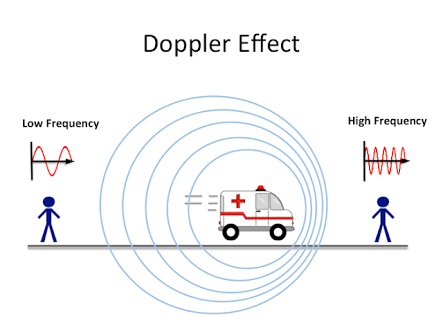
\includegraphics[width=\textwidth]{images/doppler.png}

Equations for doppler shift:

\begin{align*}
z = &\frac{\Delta f}{f} = \frac{v}{c} \\
  &\frac{\Delta \lambda}{\lambda} = -\frac{v}{c}
\end{align*}

Where $f$ is lab frequency (baseline frequency), and $\lambda$ is the lab wavelength. $v$ is the recession speed (how fast the object is travelling away from you relatively), and $c$ is the (base) speed of the wave.

\textbf{$v$ is the speed the object is travelling \textit{away} from you.}

The reason $\frac{v}{c}$ is -ve in the second equation is because the wavelength increases when travelling away, whereas the frequency would decrease.

The doppler effect can be used to work out how fast objects are moving away from us in space, as they are moving so fast that their light is red/blue shifted. From this, we can also tell how fast the universe is expanding.

We can also use this method to work out the rotational speed of a star, as one side will be slightly blue shiftd, the other will be red shifted.

Also, it can be used to figure out the speed of the orbits of binary stars, which can then be used to find a whole bunch of other stuff too. This is useful when you cannot resolve the binary system with a telescope.

\subsubsection{Spectroscopic Binary (Binary systems that cannot be resolved)}

When we cannot resolve a binary star system using a telescope, we use this method.

We use the spectral lines of each star to measure how much each star is red/blue shifted.

\newpage
\begin{center}
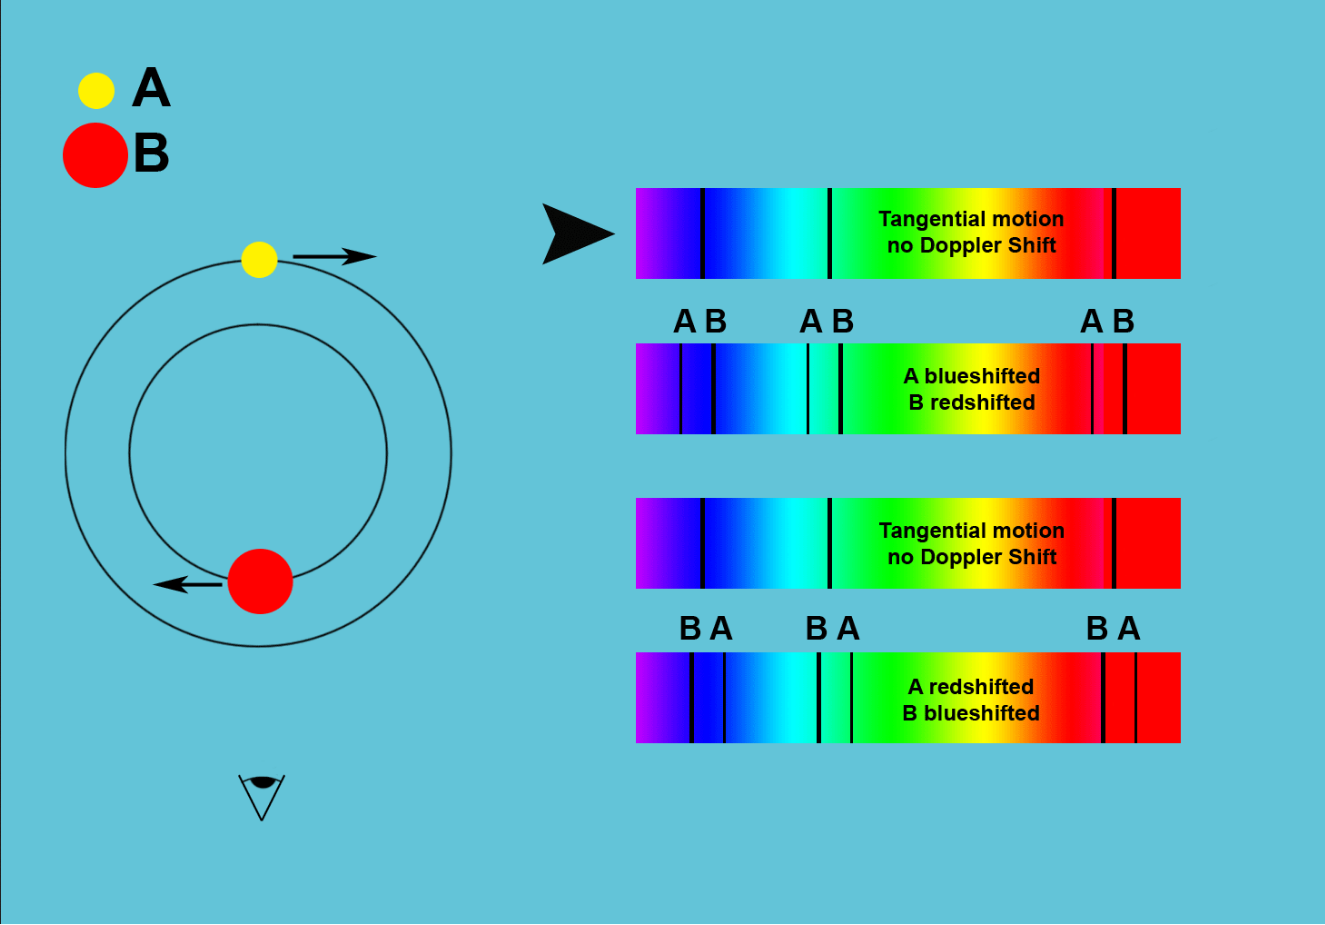
\includegraphics[height=0.4\textheight]{images/spectralBin1.png}
\end{center}

At this point, both will be at lab value wavelengths, since they are not moving towards/away from us.

\begin{center}
\includegraphics[height=0.4\textheight]{images/spectralBin2.png}
\end{center}

Now both velocities are fully towards/away, so strongest doppler effect shown. This is the value to measure to get $\Delta \lambda$.

Each star is not necessarily going to be equally doppler shifted, since one star may be bigger than the other, and hence will move slower.

\subsection{Hubble's Law}

Speed of recession of a galaxy is directly proportional to it's distance from Earth.

$$
v = Hd
$$

Where H is the Hubble constant: $65 kms^{-1} Mpc^{-1}$

\end{document}
